\documentclass[chapter.computer_science.tex]{subfiles}
\begin{document}

\section{数据库系统原理}
\subsection{绪论}
\subsubsection{基本概念}
数据是数据库中存储的基本对象,数据与其语义是不可分的,语义即对数据含义的说明。数据库是长期存储在计算机内、有组织的、可共享的大量数据的集合。
DBMS的主要功能如下:\\
\begin{enumerate}
    \item 提供数据定义语言DDL,定义数据对象。
    \item 提供数据操纵语言DML,实现对数据库的增删改查。
    \item 实现数据的组织、存储和管理,分类组织、确定数据的文件结构和存取方式,实现数据之间的联系。
    \item 数据库的运行管理。
    \item 数据库的建立和维护。
\end{enumerate}
DBS数据库系统:在计算机系统中引入数据库后的系统构成。有如下构成:数据库、数据库管理系统、应用系统、数据库管理员。数据结构化、共享性高、冗余度低且独立性高。其中的数据由DBMS统一管理和控制。数据独立性是由DBMS的二级映像功能来保证的。\\
DBAS数据库应用系统:就相当于计算机应用系统,是数据库系统与用户应用程序的结合,例如财务软件等等。\\
在数据库中使用数据模型来抽象、表示和处理现实世界中的事物。其组成要素有:数据结构、数据操作和完整性约束。数据模型分为概念模型、逻辑模型和物理模型。概念模型,即按用户的观点对数据和信息的建模,用于数据库设计。逻辑模式包括网状模型、层次模型、关系模型等,是按计算机系统的观点对数据建模,用于DBMS的实现。物理模型是对数据最底层的抽象,即在磁盘或磁带上的存储方式和存取方法。\\
在E-R图中,用矩形表示实体名(比如学生),用椭圆表示属性(比如姓名和学号),用菱形来表示联系,菱形框内写明联系名,然后在无向边中标注联系的类型。其中联系也可以具有属性:
\begin{figure}[H]
    \centering
    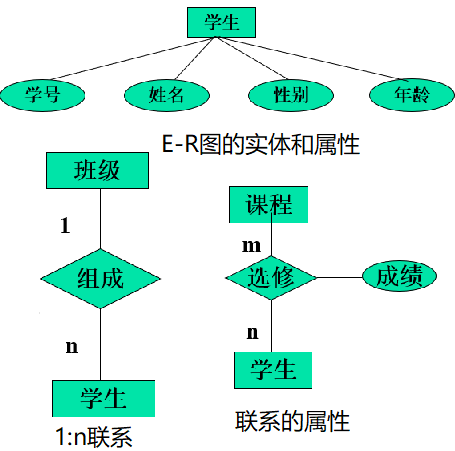
\includegraphics[scale=0.75]{./images/0019.png}
    \caption{E-R图的表示}
\end{figure}

\subsubsection{数据模型}
\begin{enumerate}
    \item 格式化模型
        \begin{enumerate}
            \item 层次模型:以树形结构来表示实体和实体间的联系,如图,其也有根节点和叶子结点等等,其只能直接处理一对多的实体联系,任何记录只有按其路径查看时,才能显示出其全部的意义,子女记录不能脱离双亲记录而单独存在。如果是多对多的话,需要将多对多分拆成多个一对多然后用层次模型表示。其查询效率高,性能优于关系模型,且不低于网状模型。
                \begin{figure}[H]
                    \centering
                    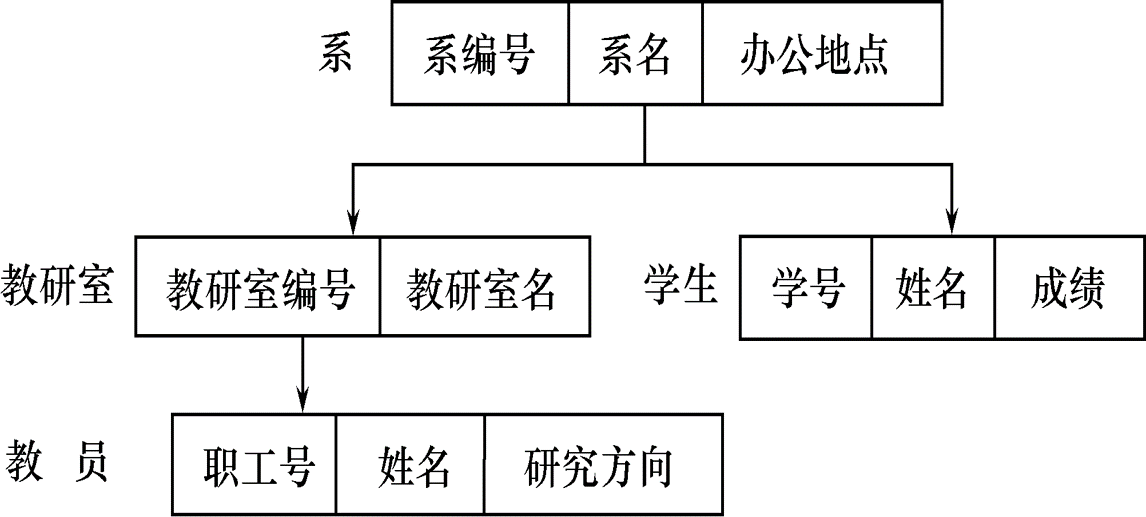
\includegraphics[scale=0.5]{./images/0020.png}
                    \caption{层次模型}
                \end{figure}
            \item 网状模型:允许一个以上的结点无双亲,且一个结点可以有多于一个的双亲。由此可见,层次模型实际上是网状模型的一个特例。网状模型的结构比较复杂,随着应用环境的扩大,数据库结构就变得愈发复杂,不利于用户的最终掌握。如下图:
                \begin{figure}[H]
                    \centering
                    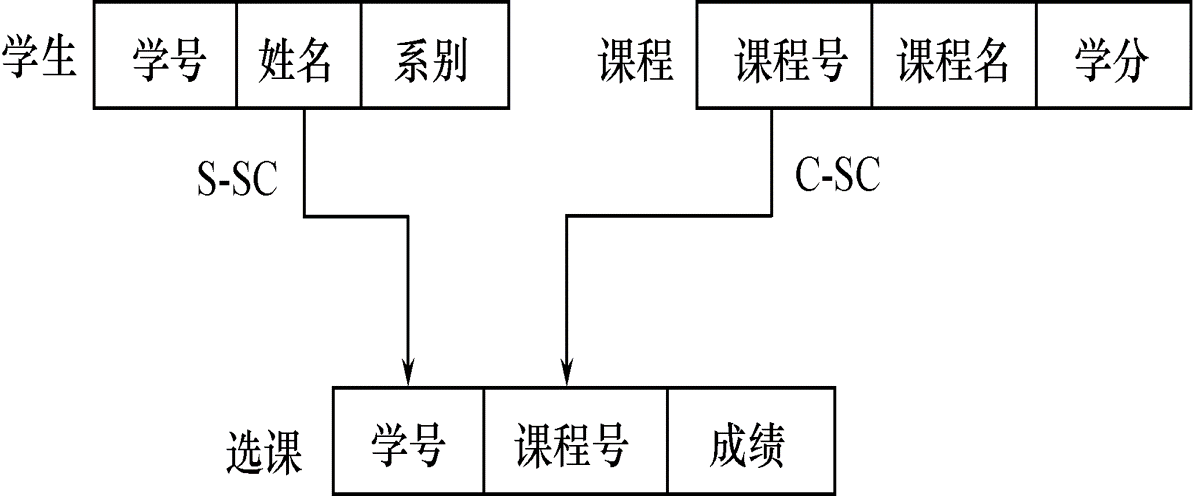
\includegraphics[scale=0.5]{./images/0021.png}
                    \caption{网状模型}
                \end{figure}
        \end{enumerate}
    \item 关系模型:关系模型下数据的逻辑结构是一张二维表,由行和列组成。其中,关系必须是规范化的,每一个分量必须是一个不可分的数据项,不允许表中有表。例如下图中的工资就是一个可分的数据项,所以其不符合关系模型的要求。关系模型中实体和各类的联系都用关系来表示,其概念单一,可描述一对一、一对多和多对多的联系,具有更高的数据独立性。
        \begin{figure}[H]
            \centering
            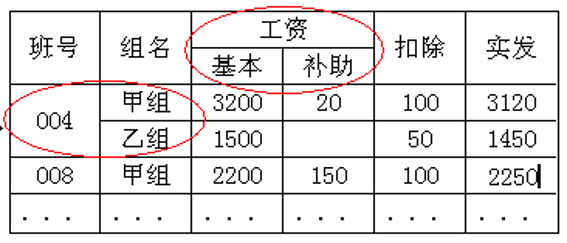
\includegraphics[scale=0.5]{./images/0022.png}
            \caption{表中有表的实例}
        \end{figure}
\end{enumerate}
\subsubsection{数据库的系统结构}
提到了一种叫做模式(schema)的概念,一般说的模式,指的是逻辑模式,是对数据库中全体数据的逻辑结构和特征的描述。{\bfseries 一个数据库只有一个模式}。其实就相当于数据库中所有表的结构的一个汇总。\\
\begin{enumerate}
    \item 外模式:亦称子模式或用户模式,是对局部数据的逻辑结构和特征的描述,通常是模式的子集。可以将其看做视图。{\bfseries 同一外模式可以被多个应用程序所使用,但一个应用程序只能使用一个外模式}。
    \item 内模式:也称存储模式,是物理结构和存储方式的表述。{\bfseries 一个数据库只有一个内模式}。
\end{enumerate}
一般数据库系统一般采用三级模式结构:
\begin{figure}[H]
    \centering
    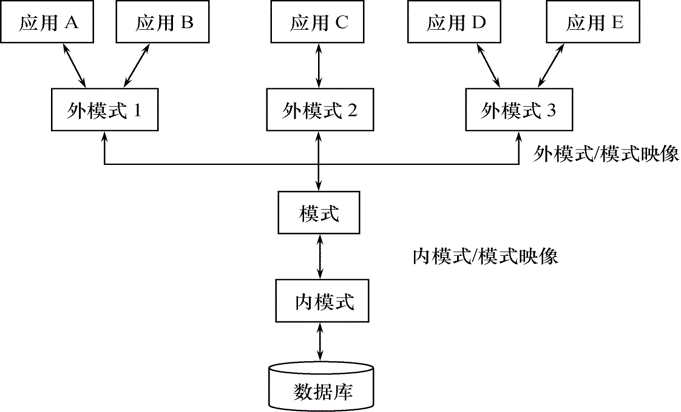
\includegraphics[scale=0.5]{./images/0023.png}
    \caption{数据库系统的三级模式结构}
\end{figure}
\begin{figure}[H]
    \centering
    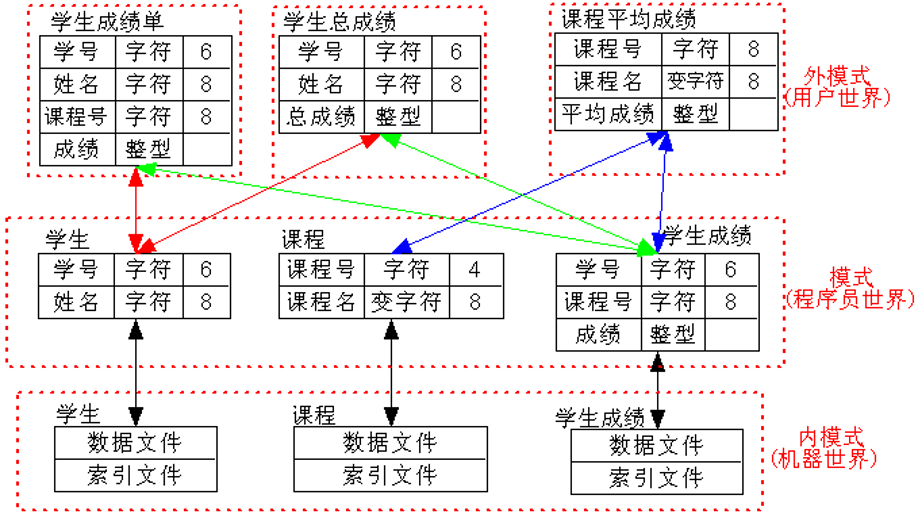
\includegraphics[scale=0.5]{./images/0024.png}
    \caption{外模式、模式与内模式}
\end{figure}

\subsection{关系数据库}
$ D_1 \times D_2 \times \cdots \times D_n $(笛卡尔积)的子集叫做在域$ D_1, D_2, \cdots, D_n $上的关系。表示为$ R(D_1, D_2,\cdots D_n) $。其中n为关系的度。说是子集的原因是因为笛卡尔积的结果不一定都是有意义的,比如$ D_1 $代表研究生导师集合,$ D_2  $代表专业集合,$ D_3 $代表学生集合,假设导师与专业是1:1的关系,与研究生是1:n的关系,那么$ D_1, D_2, D_3 $的笛卡尔积就没有实际的意义,所以说此处关系的定义实则为笛卡尔积结果中有实际意义的集合。广义笛卡尔积的计算如下:\\
\begin{figure}[H]
    \centering
    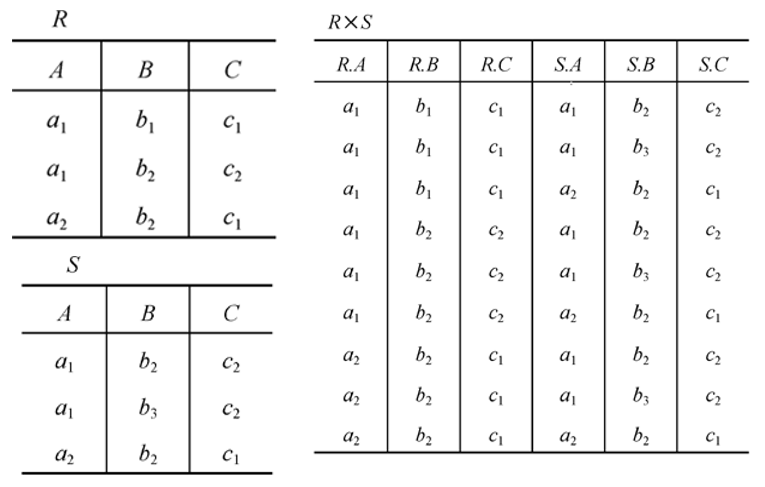
\includegraphics[scale=0.25]{./images/0025.png}
    \caption{广义笛卡尔积的计算}
\end{figure}
\subsubsection{关系运算}
选择:$ \sigma_F(R)=\{t | t \in R \cap F(t) = \text{'true'}\} $,其中F为选择的条件。例如在关系R中选出A小于5且C等于7的,即:\\
\begin{figure}[H]
    \centering
    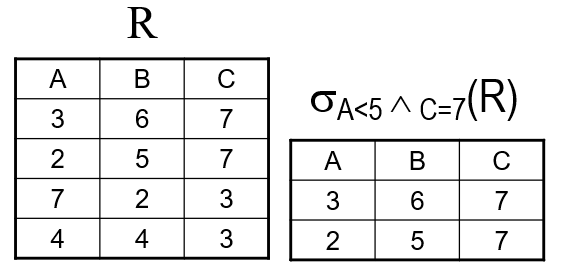
\includegraphics[scale=0.25]{./images/0026.png}
    \caption{$ \sigma_{A<5 \cap C=7}(R) $}
\end{figure}
投影:$ \Pi_A(R)=\{ t[A] | t \in R \}, A \subseteq R $,其中A为R的属性列。其实就是选R中的几列组成一个视图,需要注意的就是{\bfseries 投影的结果需要去除重复的行},例如:\\
\begin{figure}[H]
    \centering
    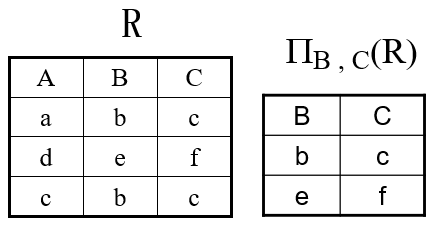
\includegraphics[scale=0.25]{./images/0027.png}
    \caption{$ \Pi_{B,C}(R) $}
\end{figure}
连接:连接操作由两步组成,第一步求两个关系的广义笛卡尔积,第二步在所求得的笛卡尔积中按条件选取满足一定条件的元组,即:$ \mathop{R \Join S}\limits_{A \theta B}=\sigma_{R.A \theta S.B}(R \times S) $,例如:\\
\begin{figure}[H]
    \centering
    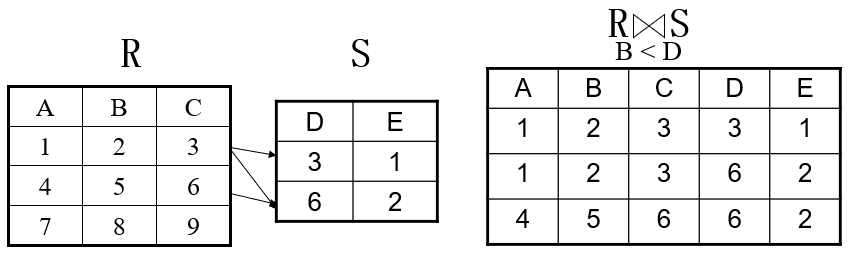
\includegraphics[scale=0.25]{./images/0028.png}
    \caption{$ \mathop{R \Join S}\limits_{B<D} $}
\end{figure}
其中$ \theta $为等号的连接运算称为{\bfseries 等值连接},即从关系R与S的广义笛卡尔积中选取A, B属性值相等的元素。{\bfseries 自然连接}是当R和S具有相同的属性组,且连接的运算符为等号,并且在连接结果中去掉重复的属性组。\\
\begin{figure}[H]
    \centering
    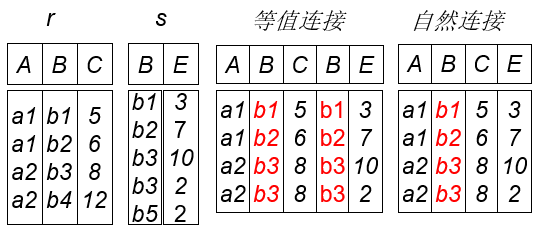
\includegraphics[scale=0.25]{./images/0029.png}
    \caption{等值连接和自然连接}
\end{figure}
外连接就是把连接中所舍弃的元组也保存在结果集中,而在其他属性上填充NULL。左外连接和右外连接即分别只保存左边关系或右边关系中要舍弃的元素,如图:\\
\begin{figure}[H]
    \centering
    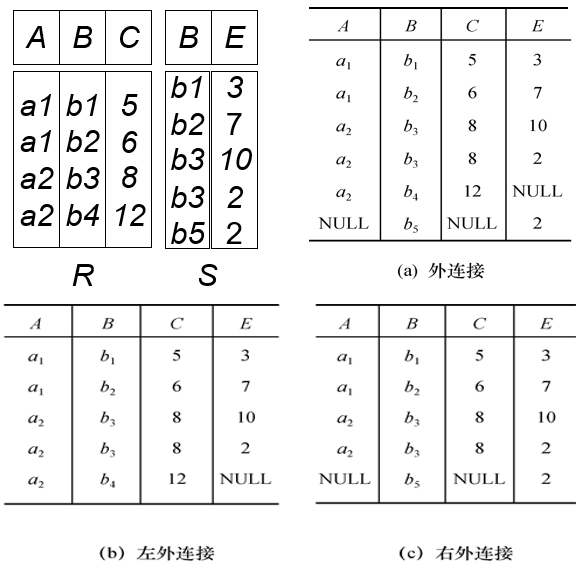
\includegraphics[scale=0.25]{./images/0030.png}
    \caption{外连接、左外连接和右外连接}
\end{figure}
可以使用如此方法来理解上文中所述的外连接,首先,我们先写出其自然连接的结果,就有了外连接结果中的前4行,然后我们再来看R和S,R中有$ a_2,b_4,12 $在S中找不到对应的连接对象,同样S中有$ b_5,2 $在R中找不到对应的连接对象,因此,将这两行分别加上NULL,填入外连接的结果集中。同理,如果只保存R或S中要舍弃的元素就有了左外连接和右外连接的结果。\\
象集:说白了就是选出其中的一列作为新的关系而单独存在。除运算这个比较难以表述:\\
\begin{figure}[H]
    \centering
    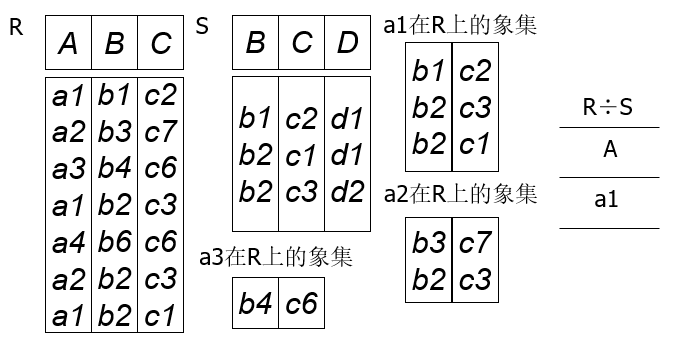
\includegraphics[scale=0.25]{./images/0031.png}
    \caption{除运算}
\end{figure}
在关系R中,A可以取四个值\{a1,a2,a3,a4\},分别求出这四个值的象集如图,然后求出S在(B,C)上的投影为\{(b1,c2),(b2,c3),(b2,c1)\},显然只有R的象集$ a_1 $包含S在(B,C)属性组上的投影上,所以 $ R \div S=\{a_1\} $。\\
关系具有如下三类完整性:实体完整性、参照完整性和用户定义完整性,其中{\bfseries 关系必须满足实体完整性和参照完整性}。实体完整性的例子就比如主键唯一且不能取空值。参照完整性的例子就比如外键。

\subsection{数据库的转储与恢复}
\subsubsection{静态转储与动态转储}
\begin{enumerate}
    \item 静态转储:转储时系统中无运行事务且处于一致性状态且转储期间不允许对数据库进行任何的存取、修改活动。
    \item 动态转储:转储期间允许与用户事务并发进行且转储期间允许对数据库进行存取和修改,有个缺点就是不能保证副本中数据的正确有效。在进行动态转储时,需要把动态转储期间各事务对数据库的修改活动登记下来建立日志文件,然后{\bfseries 后备副本加上日志文件}才能把数据库恢复到某一时刻的正确状态。登记日志的时候{\bfseries 必须先写日志文件后写数据库}。
\end{enumerate}
\subsubsection{先写日志文件后写数据库的原因}
\begin{enumerate}
    \item 如果先写了数据库修改,而在日志文件中没有登记下这个修改,则以后就无法恢复这个修改了。
    \item 如果先写日志,但没有修改数据库,按日志文件恢复时只不过是多执行一次不必要的UNDO操作,并不会影响数据库的正确性。
\end{enumerate}
\subsubsection{系统故障恢复的步骤}
\begin{enumerate}
    \item 首先{\bfseries 正向扫描日志文件}:将在故障发生前已经提交的事务(既有BEGIN TRANSACTION记录又有COMMIT记录)加入{\bfseries 重做队列}。将故障发生时尚未完成的事务(只有BEGIN TRANSACTION记录而没有COMMIT记录)加入{\bfseries 撤销队列}。
    \item 对撤销队列中的事物进行撤销处理:{\bfseries 反向扫描日志文件},对每个撤销事物执行逆操作,将更新前的值写入数据库。
    \item 对重做队列的事物进行重做处理:{\bfseries 正向扫描日志文件},对每个重做事务重新执行登记操作,将日志记录的更新后的值写入数据库。
\end{enumerate}

\subsection{关系数据理论}
\subsubsection{函数依赖}
函数依赖:就类似于数学上函数的定义一样,$ Y=f(X) $即称为X函数确定Y,或者Y函数依赖于X,记作$ X \rightarrow Y $。X称为这个函数依赖的决定属性组(Determinant)。其真正想说明的是,像数学上定义的函数一样,X和Y是一一对应的关系。\\
\begin{enumerate}
    \item 对于$ X \rightarrow Y $,且$ Y \nsubseteq X $,则称$ X \rightarrow Y $为非平凡函数依赖。
    \item 对于$ X \rightarrow Y $,且$ Y \subseteq X $,则称$ X \rightarrow Y $为平凡函数依赖。
\end{enumerate}
同样,如果$ X \rightarrow Y $,且对于X的任意一个真子集$ X' $都有$ X' \nrightarrow Y $,则称Y对X{\bfseries 完全函数依赖},否则称为部分函数依赖。
\subsubsection{规范化}
如果一个关系模式R中的所有属性都是不可分的基本数据项,则R为1NF。{\bfseries 1NF为关系数据库的基本要求,不满足1NF的不能称为关系数据库}。若一个关系为1NF且每一个非主属性完全函数依赖于码(码和非主属性之前有一一对应,而且是完全对应的关系,就像一个主键可以唯一确定一行这样),则R为2NF。在下列2NF的示例中,还存在一层传递依赖关系即:学号->专业->宿舍楼号,此时如果将这层传递依赖关系消除,则可以得到3NF,在3NF中,每一个非主属性既不部分依赖于码也不传递依赖于码。在BCNF中,没有任何属性完全函数依赖于非码的任何一组属性,所有的非主属性对每一个码都是完全函数依赖,所有的主属性对每一个不包含它的码也是完全函数依赖。\\
\begin{minted}{sql}
    # 1NF
    # 学号, 专业, 宿舍楼号, 课程号, 课程成绩
    S-L-C(Sno, Sdept, Sloc, Cno, Grade)
    # 2NF
    SC(Sno, Cno, Grade)
  	S-L(Sno, Sdept, Sloc)
    # 3NF
    SC(Sno, Cno, Grade)
    S-D(Sno, Sdept)
    D-L(Sdept, Sloc)
    #
\end{minted}

\end{document}
